\documentclass[xcolor=pdftex,dvipsnames,table,usenames,11pt]{beamer}
%\documentclass[xcolor=pdftex,dvipsnames,table]{beamer}

\usetheme{Berlin}
\usecolortheme{beaver}
\usepackage{mathpazo}
\usepackage{tgpagella}
%\usepackage[latin1]{inputenc}
\usepackage{amsmath}
\usepackage{mathabx}
%\usepackage{amsfonts}
\usepackage{amssymb}
\usepackage{amsthm}
\usepackage{tikz}
\usetikzlibrary{positioning}
\usepackage{tikzpagenodes}
\usepackage{bbm}
\usepackage{bm}
\usepackage{textcomp}
\usepackage{appendix}
\usepackage{graphicx}

\newcommand{\sub}[1]{\ensuremath{_\mathrm{#1}}}

\usepackage[backend=bibtex]{biblatex}
\bibliography{../../../../../Mendeley/bibtex/OtherResearch-AuroraBorealis}

\usepackage{array}
\usepackage{multicol}				% multi-column layout
\newenvironment{equations}{\equation\aligned}{\endaligned\endequation} % Combines splitting and alignment

\newcommand{\dd}[2]{\frac{\mathrm{d}#1}{\mathrm{d}#2}}
\newcommand{\pp}[2]{\frac{\partial #1}{\partial #2}}
\newcommand\encircle[1]{%
  \tikz[baseline=(X.base)] 
    \node (X) [draw, shape=circle, inner sep=0] {\strut #1};}
\usepackage{scrextend}
\changefontsizes{11pt}
\usefonttheme{professionalfonts} % using non standard fonts for beamer
\usefonttheme{serif} % default family is serif
\renewcommand{\vec}[1]{\ensuremath{\mathbf{#1}}}
% Special symbols
\DeclareMathOperator*{\schmidt}{Sc}
\DeclareMathOperator*{\pH}{pH}
\DeclareMathOperator*{\re}{Re}
\DeclareMathOperator*{\St}{St}
\DeclareMathOperator*{\Sc}{Sc}
\providecommand{\bigO}[1]{\ensuremath{\mathop{}\mathopen{}\mathcal{O}\mathopen{}\left(#1\right)}}
% Chemistry




\newcommand{\anitem}{\item[-]}
\setbeamercolor{block title}{bg=black!20,fg=black}
\def\labelitemi{--}

\setbeamertemplate{itemize item}{\color{black}-}
\setbeamertemplate{itemize subitem}{\color{black}-}
\setbeamertemplate{itemize subsubitem}{\color{black}-}


\newcommand{\subitem}[1]{\begin{itemize}\item #1\end{itemize}}






\begin{document}
%\logo{\includegraphics[height=0.4cm]{uoitlogo.pdf}}

\title{Simulating the Aurora Borealis}
\author[]{Kyle Mills}
\institute[University of Ontario Institute of Technology]{University of Ontario Institute of Technology}
\date[ ] % (optional, should be abbreviation of conference name)
{\footnotesize{Mathematical Modelling, Winter 2015}}

\setbeamertemplate{navigation symbols}{}


%\definecolor{beamer@blendedblue}{rgb}{0.137,0.466,0.741}
%\setbeamercolor*{palette tertiary}{use=structure,fg=white,bg=black}


{ % all template changes are local to this group.
    
    \begin{frame}[plain]
        \begin{tikzpicture}[remember picture,overlay]
            \node[at=(current page.center)] {
                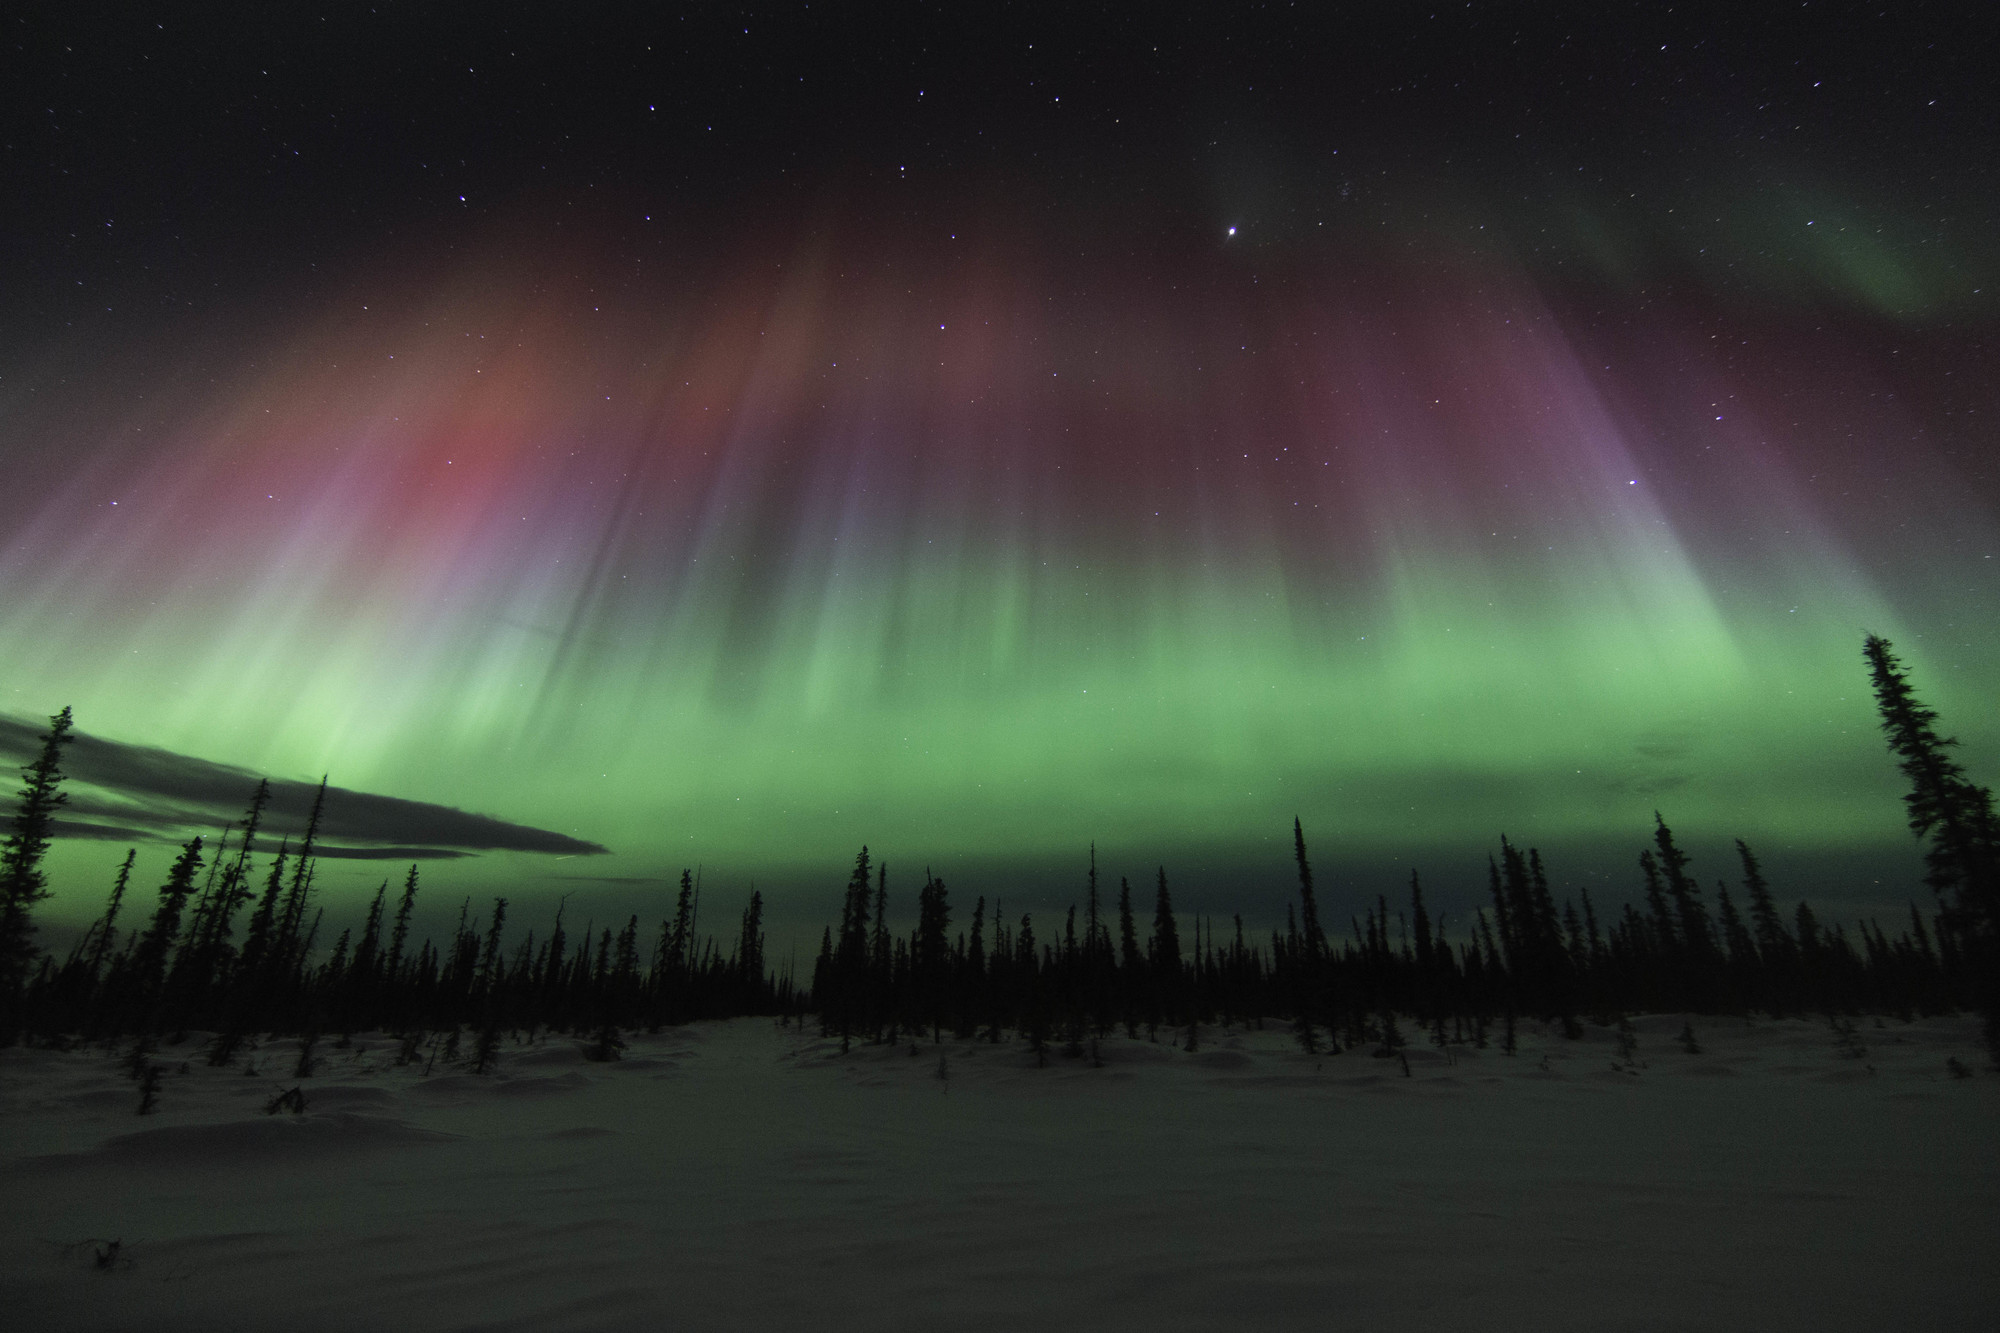
\includegraphics[width=1.5\paperwidth]{img/Aur_cover.jpg}
            };
            \begin{scope}[ fill opacity=0.5]
            \fill[black] {(current page.center) circle (3.1cm) };
            \end{scope}
            \node[draw=none,text width=6cm, align=center] (title) at (current page.center) {\color{white} {\huge Simulating the\\ Aurora }};
            \node[draw=none, text width=6cm, align=center, below = 0.4cm of title] (author) {\color{white}\small Kyle Mills};
            
            \node[draw=none, text width=6cm, align=center] (course) at (current page text area.south) {\color{white}\tiny Advanced\hspace{0.3em}Topics\hspace{0.3em}in\hspace{0.3em}Computational\hspace{0.3em}Science, 2015};            
        \end{tikzpicture}
     \end{frame}
}







\section{Introduction}



\begin{frame}{What is the Aurora?}
\begin{itemize}
\item Solar wind sends charged particles (electrons) toward Earth
\item Earth's magnetic field funnels the electrons to the poles and accelerates them downward toward Earth
\item Electrons travel at high speeds (10 keV)
\begin{center}
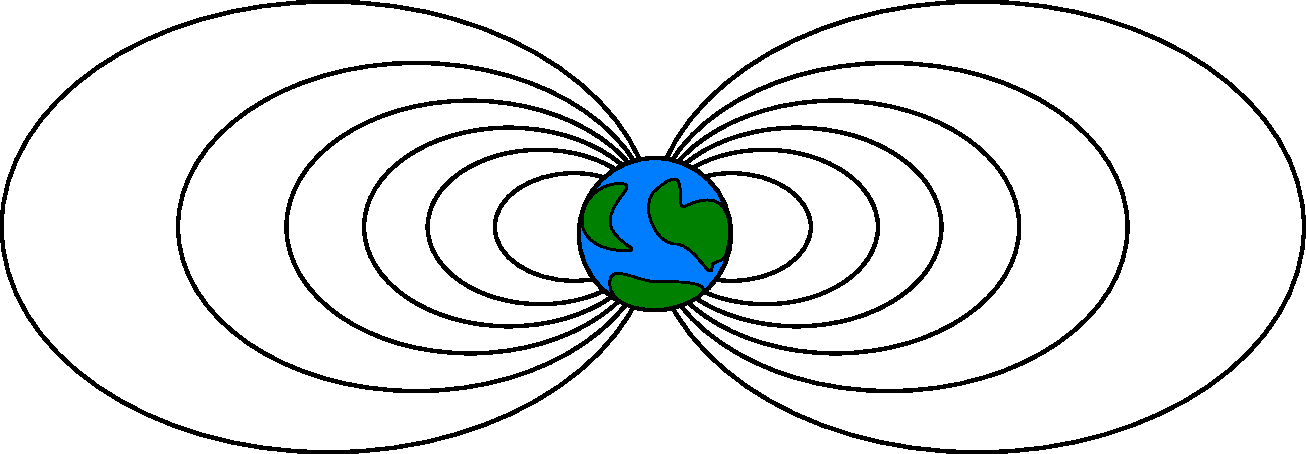
\includegraphics[width=0.5\textwidth]{img/fieldlines.pdf}
\end{center}
\end{itemize}
\end{frame}















\begin{frame}{Colours}
\begin{columns}[onlytextwidth]
  \begin{column}{0.5\textwidth}
    \begin{itemize}
    \item electrons excite atomic oxygen and nitrogen
    \item excited state decays, emits photon 
    \item wavelength depends on atom type:
    \begin{itemize}
        \item{O: red \& green}
        \item{N: blue (rare)}
    \end{itemize}
    \end{itemize}
  \end{column}
  \begin{column}{0.05\textwidth}
  \end{column}
  \begin{column}{0.5\textwidth}
    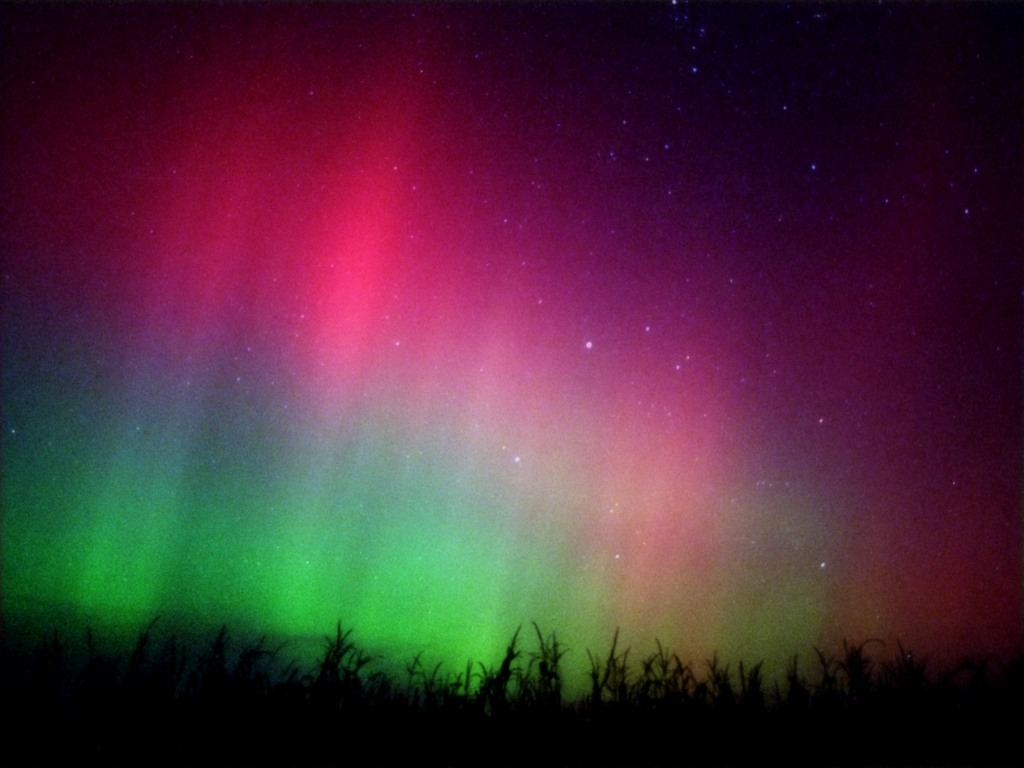
\includegraphics[width=\textwidth]{img/p4a.jpg}
  \end{column}
\end{columns}
\end{frame}






\begin{frame}{Colours}
\begin{columns}[onlytextwidth]
  \begin{column}{0.6\textwidth}
    \begin{itemize}
    \item Excited states take varying times to decay:
    \begin{itemize}
        \item Red: 100+ seconds
        \item Green: 0.5 seconds
        \item Blue: 0.01 seconds
    \end{itemize}
    \item Between excitation and emission, if atom collides with another atom, energy will be dissipated without photon emission
    \end{itemize}
  \end{column}
  \begin{column}{0.05\textwidth}
  \end{column}
  \begin{column}{0.4\textwidth}
    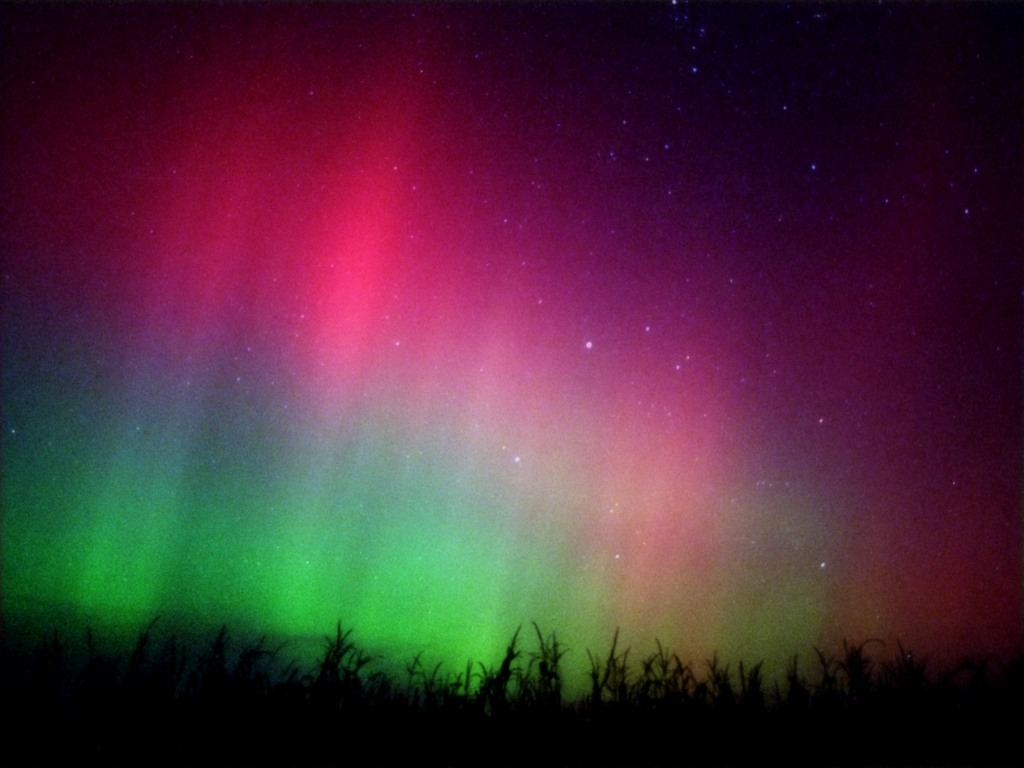
\includegraphics[width=\textwidth]{img/p4a.jpg}
  \end{column}
\end{columns} 
\begin{itemize}
    \item Long-lived photons (red) produced only in low density (high altitude)
\end{itemize}
\end{frame}










\begin{frame}{Structure}
\begin{columns}[onlytextwidth]
  \begin{column}{0.5\textwidth}

    \begin{itemize}
        \item \textbf{Swirls:} ionospheric currents, density variations
        \item \textbf{Vertical banding:} Collective electric field of the electrons
    \end{itemize}

    Aside from accelerating the particles, magnetic field has very little effect.

  \end{column}
  \begin{column}{0.05\textwidth}
  \end{column}
  \begin{column}{0.5\textwidth}
    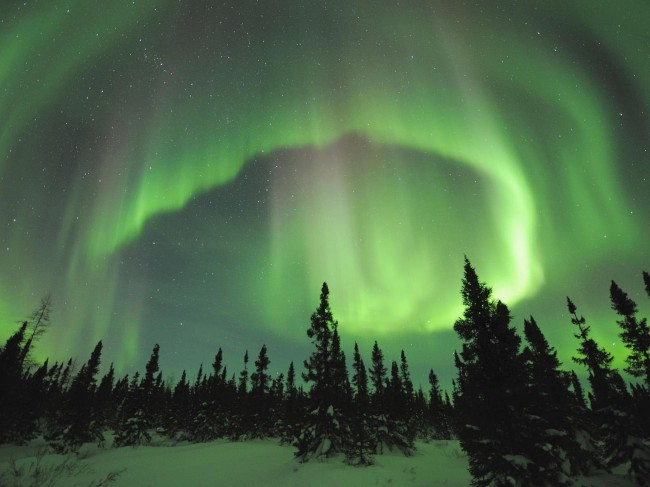
\includegraphics[width=\textwidth]{img/ab_swirls.jpg}
  \end{column}
\end{columns} 

\end{frame}













\section{The Model}



\begin{frame}{The simulation box}
\begin{columns}[onlytextwidth]
  \begin{column}{0.5\textwidth}
    \begin{itemize}
    \item $200\times 200\times 200$ simulation box (each voxel $\sim 1$ km$^3$ )
    \item Periodic boundary conditions in $x$ and $y$.
    \item Electron flux through top
    \item track the electrons as they progress through time
    \end{itemize}
  \end{column}
  \begin{column}{0.05\textwidth}
  \end{column}
  \begin{column}{0.45\textwidth}
    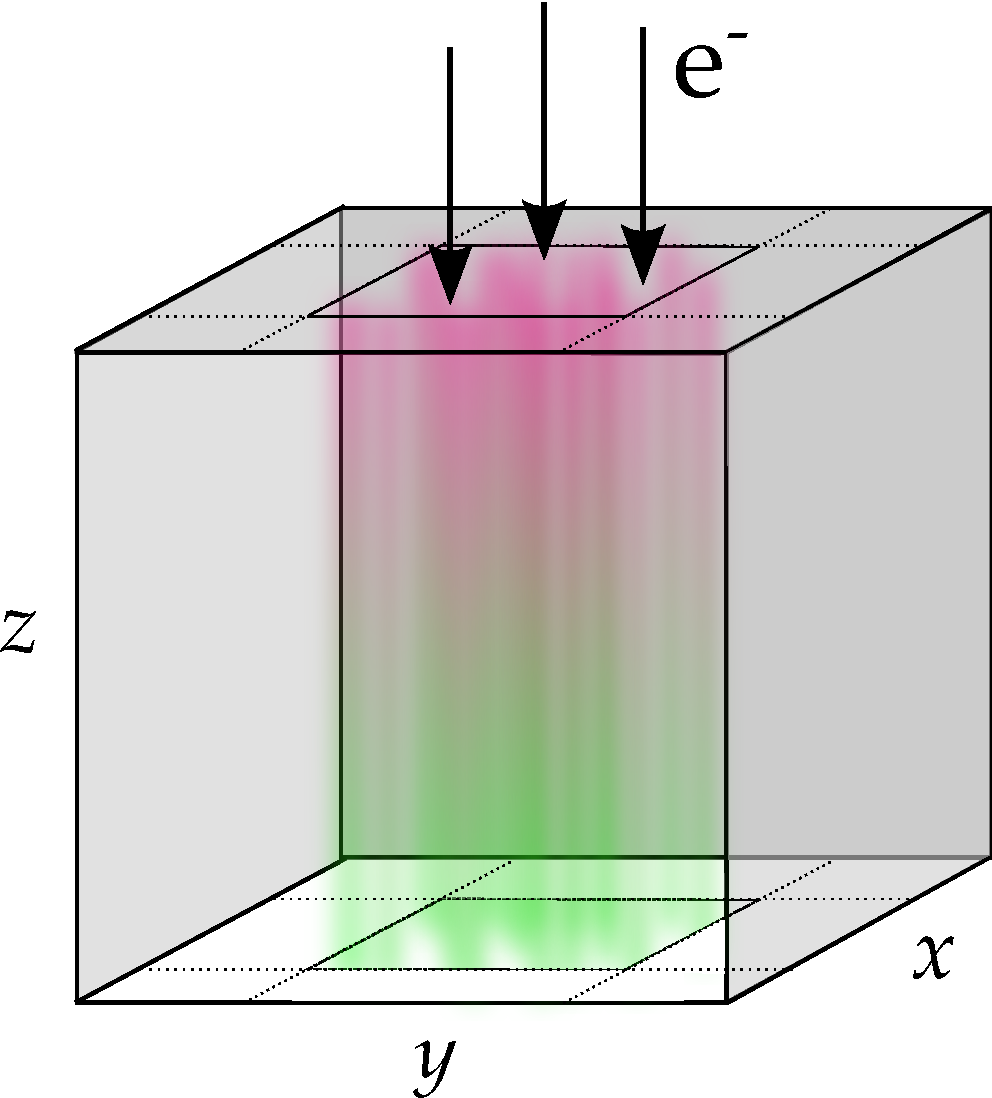
\includegraphics[width=\textwidth]{img/simulation_cell.pdf}
  \end{column}
\end{columns}
\end{frame}









\begin{frame}{Algorithm: Motion}
\begin{itemize}
\item Each (non-interacting) electron has a 
\begin{itemize}
\item position vector $\vec x$,
\item velocity vector $\vec v$,
\item force vector $\vec F$
\end{itemize}
\item External influences (e.g. \vec B, \vec E field) can interact through $\vec F$.
\pause
\item Basic Newton integration used to time-evolve electrons:
\begin{equation*}
\vec v (t + dt) = \vec v(t) + \frac{\vec F}{m} dt; \qquad \vec x(t + dt) = \vec x (t)  + \vec v(t+dt) dt .  
\end{equation*}
\end{itemize}
\end{frame}














\begin{frame}{Algorithm: ``Interaction'' with atoms}
Stochastic approach to emission
\begin{itemize}
\item \textbf{Monte Carlo:} probability of a collision depends on height (ie: $P\sub{emit} = P\sub{emit}(z)$ )
\item If there is a collision, use \textbf{Kinetic Monte Carlo} to determine if a photon is emitted, and the colour. Rates dependent on height.
\end{itemize}
\end{frame}




\begin{frame}
The colour dependence on height can be dealt with by using probability thresholds derived from observed colours.
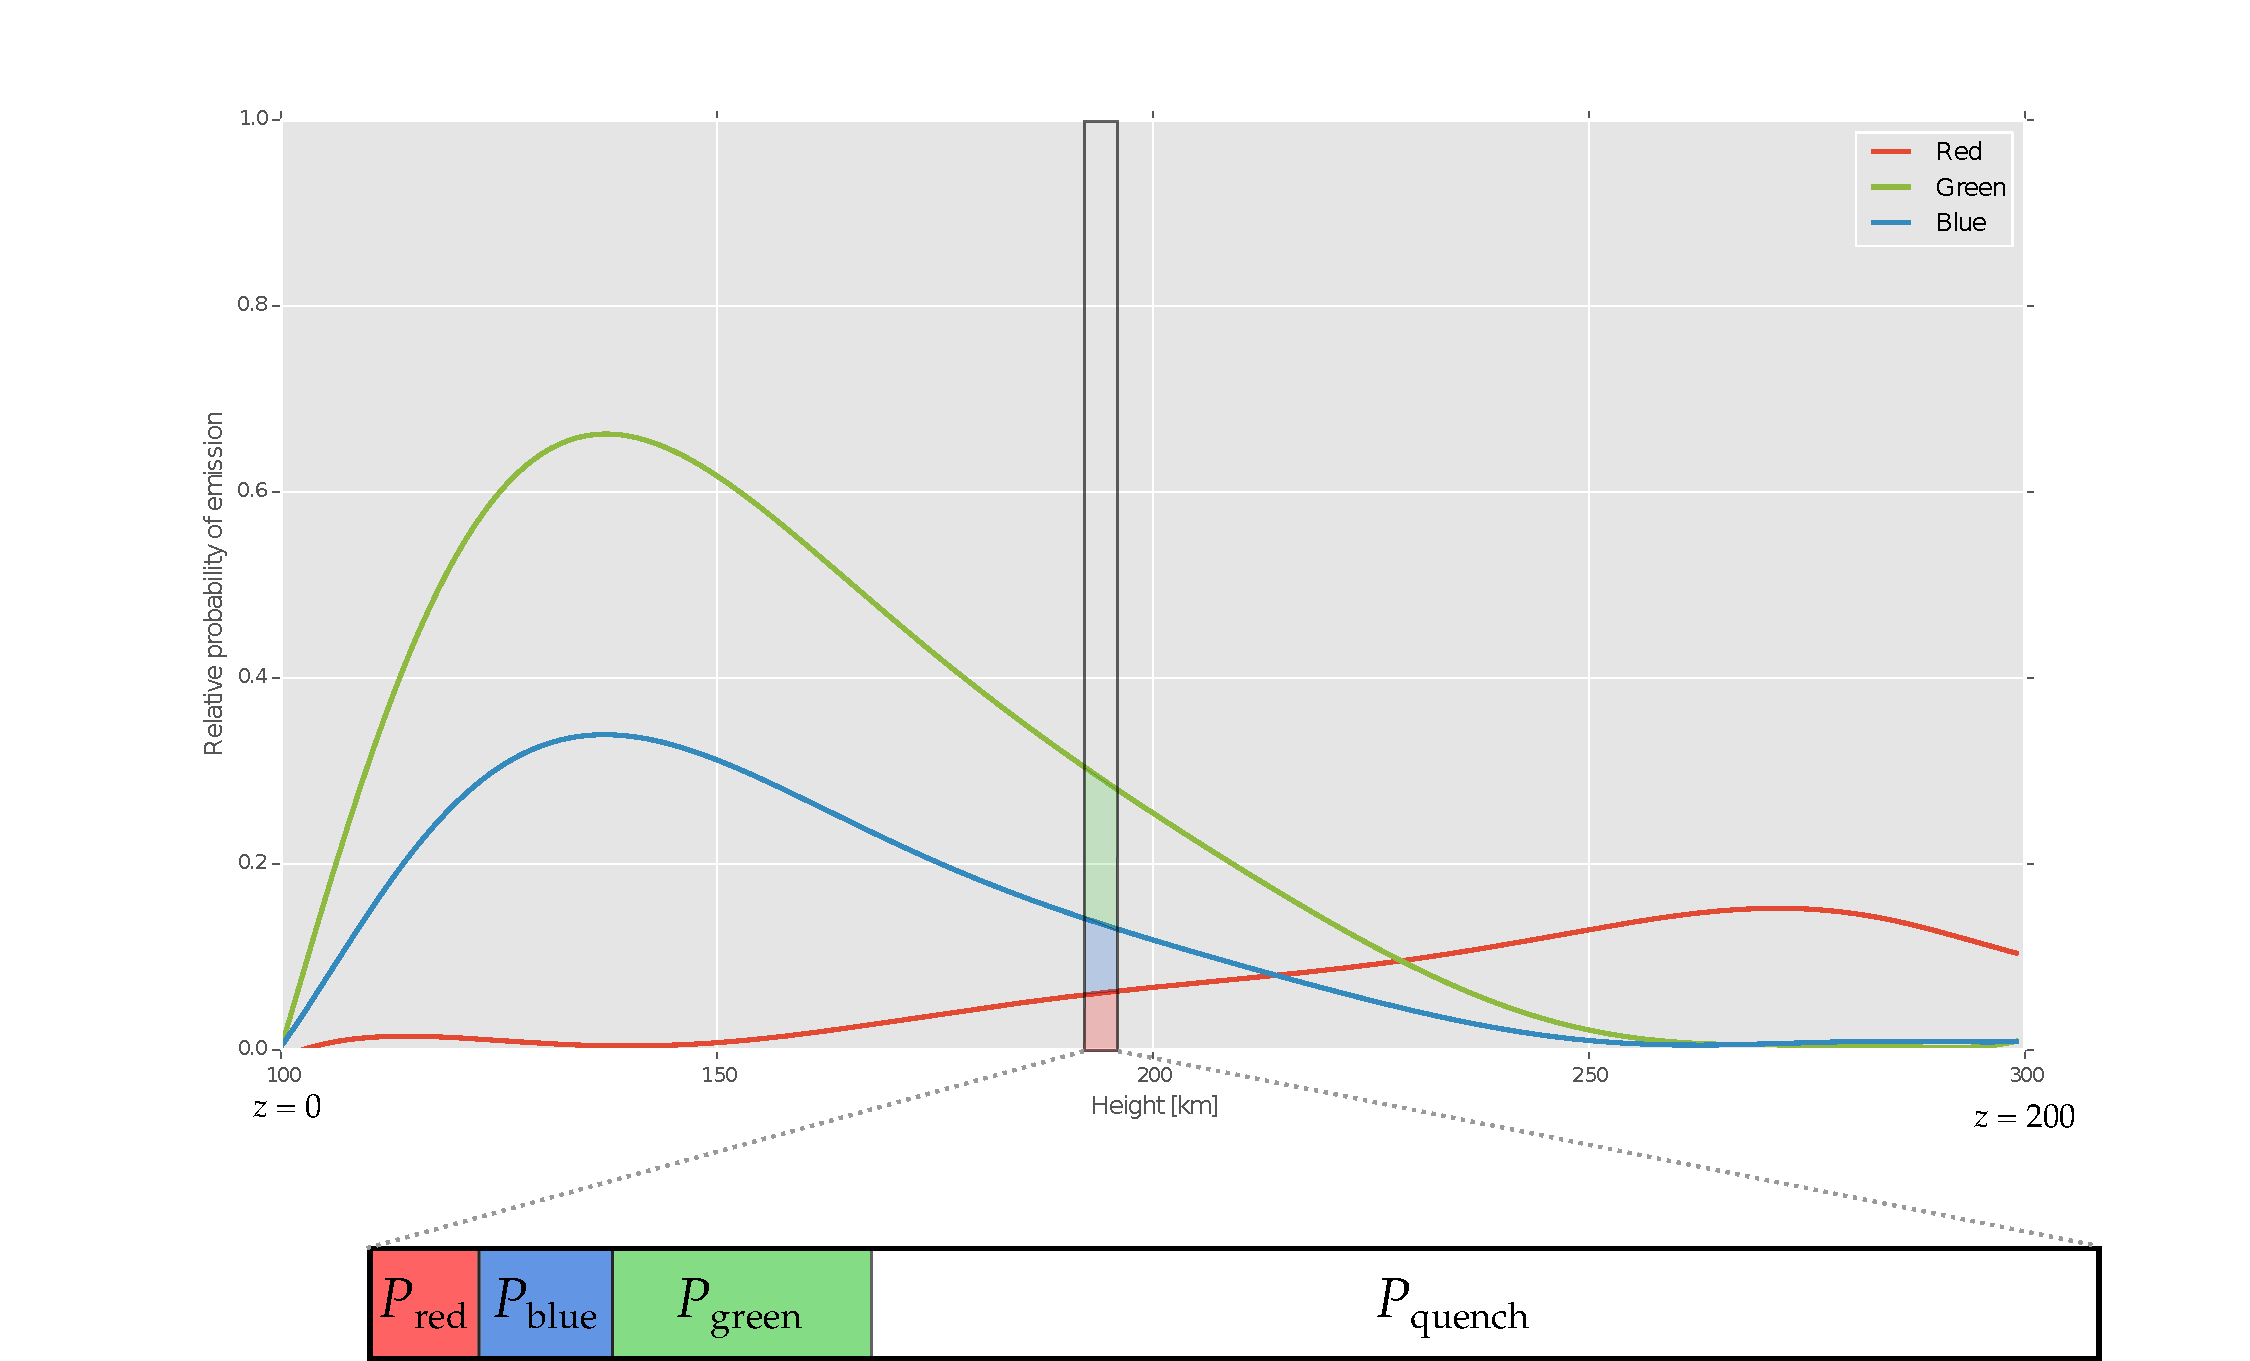
\includegraphics[width=\textwidth]{img/Earth_color_probs.pdf}\\
{\hfill \tiny data source: Baranoski [2003] }
\end{frame}






\begin{frame}{Algorithm: ``Interaction'' with atoms}
\begin{itemize}
\item If an emission occurs:
\begin{itemize}
\pause
\item increment the corresponding ``photon density'' voxel. 
\pause
\item Transfer the photon energy ($\Delta E = hc/\lambda$) from the electron to an array keeping track of energy deposition.
\end{itemize}
\pause
\item One photon intensity array per colour channel (red, green blue)
\begin{center}
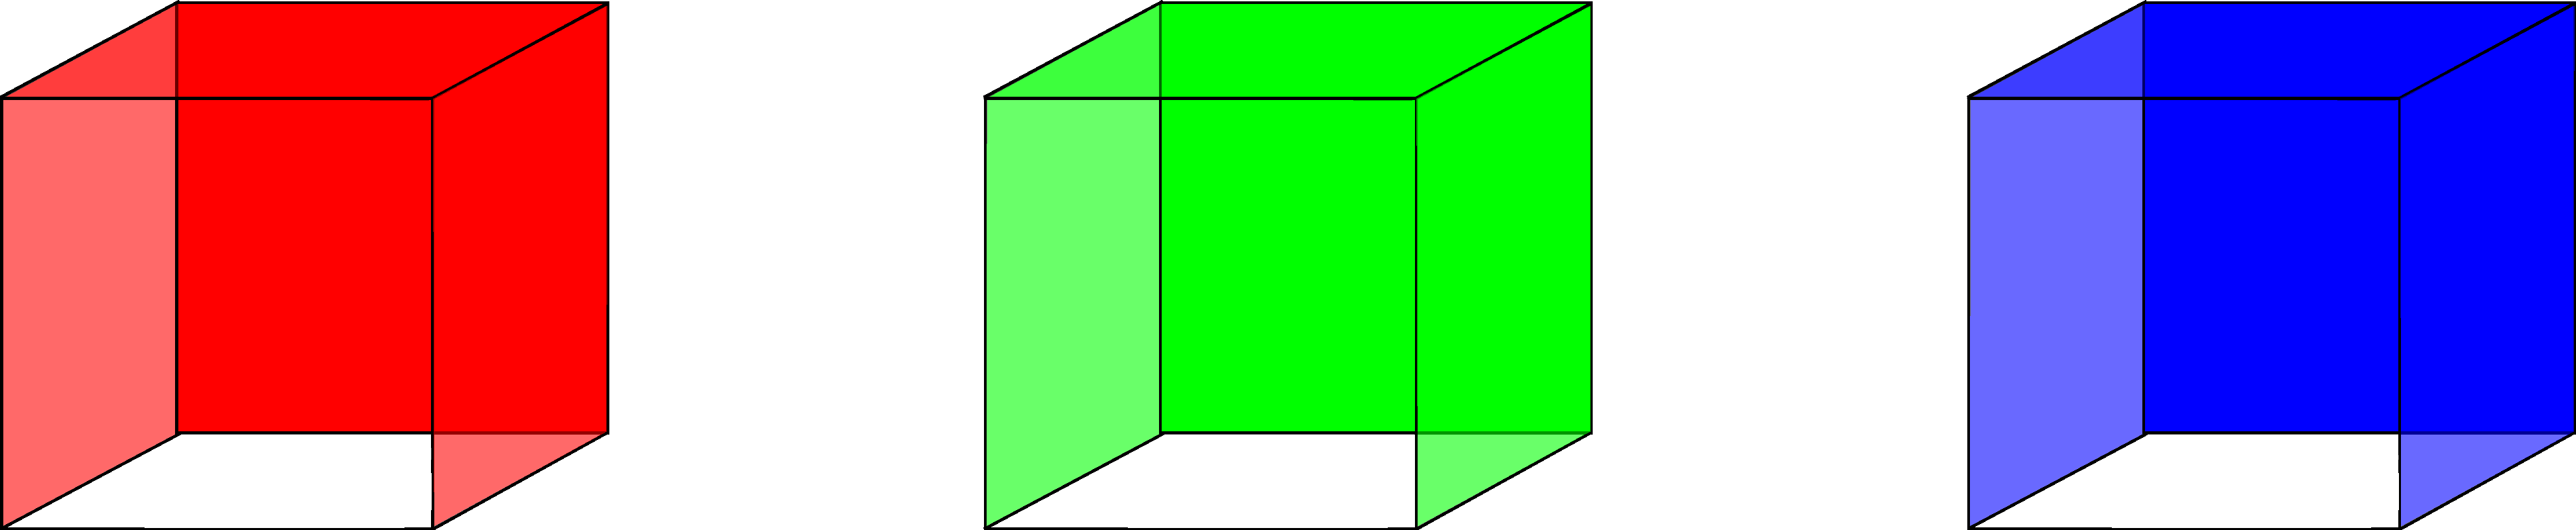
\includegraphics[width=0.8\textwidth]{img/photon_density.pdf}
\end{center}
\item Can later map this 3D data to a 2D image for visualization.
\end{itemize}
\end{frame}

















\begin{frame}{Electrostatics}
\begin{itemize}
\item Structure comes from electric field $\vec E$
\item Need to compute $\vec E$ from the charge density $\rho$.
\begin{itemize}
\item{At each timestep, compute $\rho$}
\item {Solve Poisson's equation:}
\begin{equation*}
\nabla^2\phi = -\frac{\rho}{\epsilon_0}
\end{equation*}
\item Compute $\vec E$ through 
\begin{equation*}
\vec E = -\nabla \phi
\end{equation*}


\end{itemize}

\end{itemize}
\end{frame}











\begin{frame}{Electrostatics}
\begin{itemize}
\item Electron reset if
\begin{itemize}
\item it exits box through the bottom
\item its energy falls below the energy of a photon
\end{itemize}
\end{itemize}
\end{frame}

























\begin{frame}{Electrostatics}
\begin{itemize}
\item Implemented using Fourier transforms (FFTW3).
\item Spectral methods used to directly compute $\vec E$ from $\mathcal{F}_\rho$ (the Fourier transform of $\rho$ ).
\begin{equation*}
\phi(\vec r) = \frac{1}{\epsilon_0}\int{\frac{\rho(\vec r') }{\vec r^2  } \mathrm{d} ^3\vec r} = -\frac{1}{2\pi\epsilon_0}\int{ \frac{\mathcal{F}_\rho (\vec k)}{\vec k^2}e^{i\vec k\cdot\vec r }\mathrm{d}^3\vec k    }
\end{equation*}
\begin{equation*}
\vec E = -\nabla \phi  = \frac{i}{2\pi\epsilon_0}\int{   \frac{\vec k \mathcal{F}_\rho (\vec k)}{\vec k \cdot \vec k}e^{i\vec k\cdot\vec r }\mathrm{d}^3\vec k       }
\end{equation*}
\end{itemize}
\end{frame}











\begin{frame}{Electrostatics}
	\begin{itemize}
		\item Electrons interact with $\vec E$ through the Lorentz force
		\begin{equation*}
		\vec F = q(\vec E + \vec v \times \vec B)
		\end{equation*}
		\item \vec B taken as constant field in $-y$ direction (\vec B points toward North Pole)
\end{itemize}
\end{frame}













\section{Results}

\begin{frame}{Results}
\begin{columns}[onlytextwidth]
  \begin{column}{0.5\textwidth}
  Baranoski uses a complicated visual rendering procedure:
  \begin{itemize}
  \item perspective projection to trace photons to Earth-bound observer
  \item Gaussian kernel convolution to blur the images to smooth it out
  \end{itemize}
  \end{column}
  \begin{column}{0.05\textwidth}
  \end{column}
  \begin{column}{0.5\textwidth}
    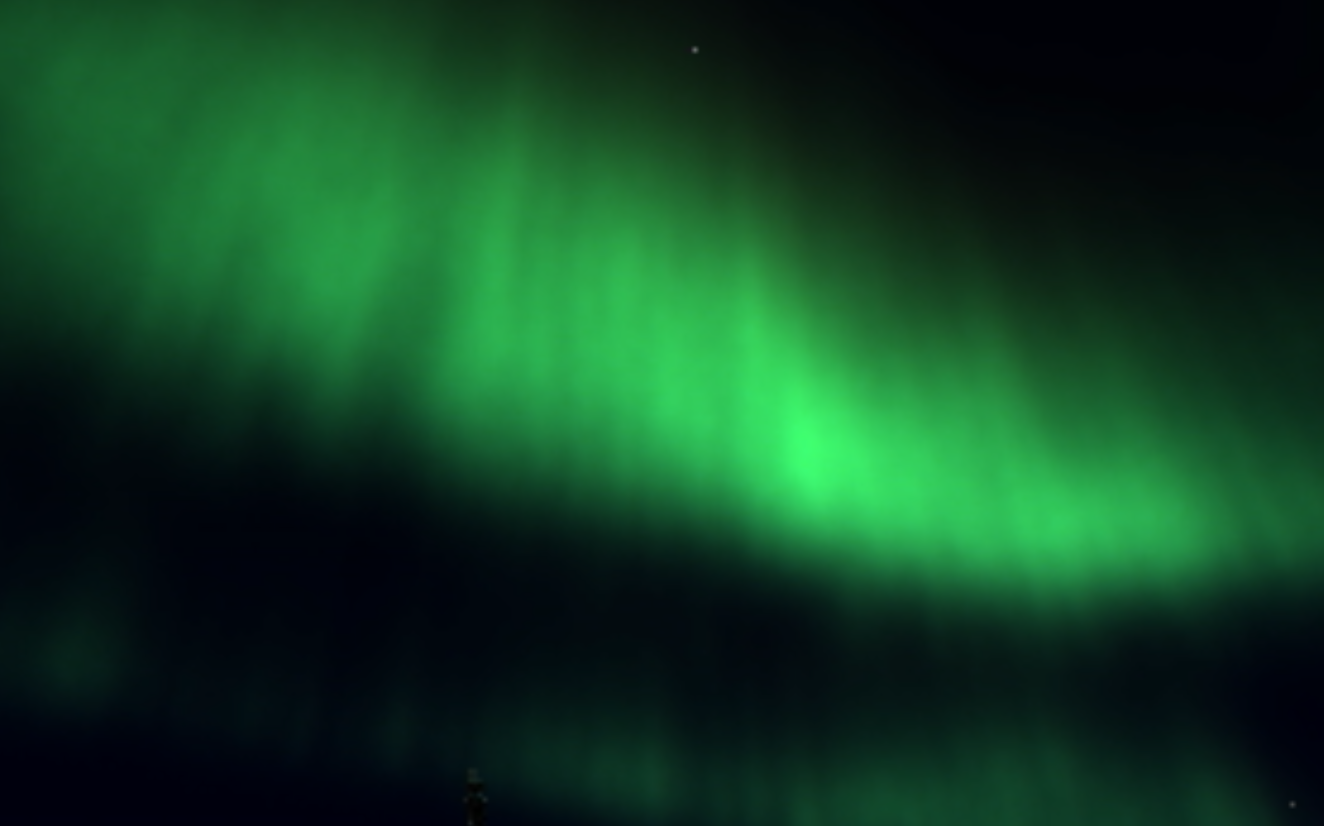
\includegraphics[width=\textwidth]{img/baran_results.png}\\
	\hfill { \tiny Baranoski [2003]}
  \end{column}
\end{columns} 
\end{frame}













\begin{frame}
\begin{columns}[onlytextwidth]
  \begin{column}{0.5\textwidth}
  I use a 
  \begin{itemize}
  \item direct orthographic projection
  \item photon brightness decays as $1/x^2$
  \end{itemize}
  \end{column}
  \begin{column}{0.05\textwidth}
  \end{column}
  \begin{column}{0.5\textwidth}
    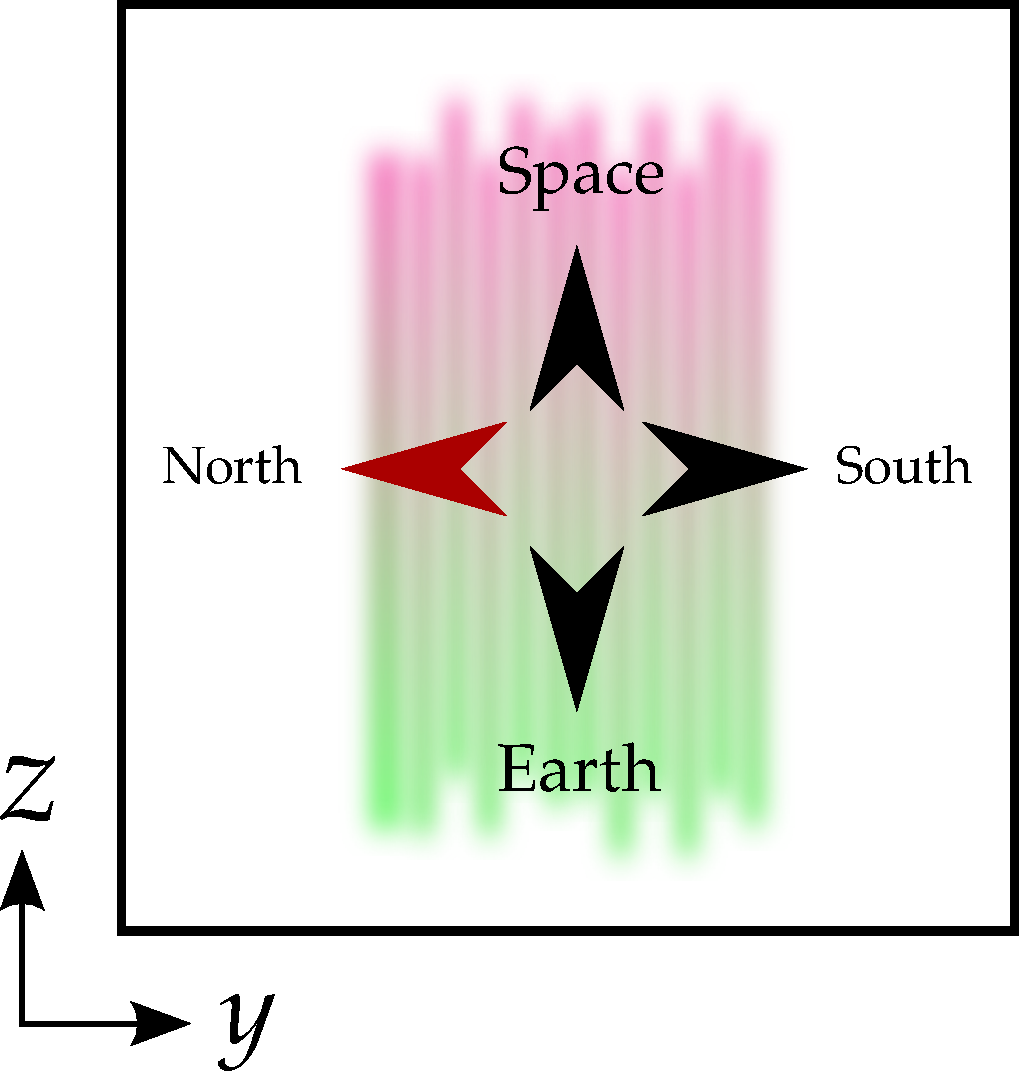
\includegraphics[width=\textwidth]{img/projection.pdf}\\
	\hfill { \tiny My projection}
  \end{column}
\end{columns} 
\end{frame}








\begin{frame}
\begin{center}
\href{run:/home/kmills/Dropbox/3.AdvancedTopics/AdvancedTopics/project/AuroraSim/presentation/vid/Earth_1.mkv}{
	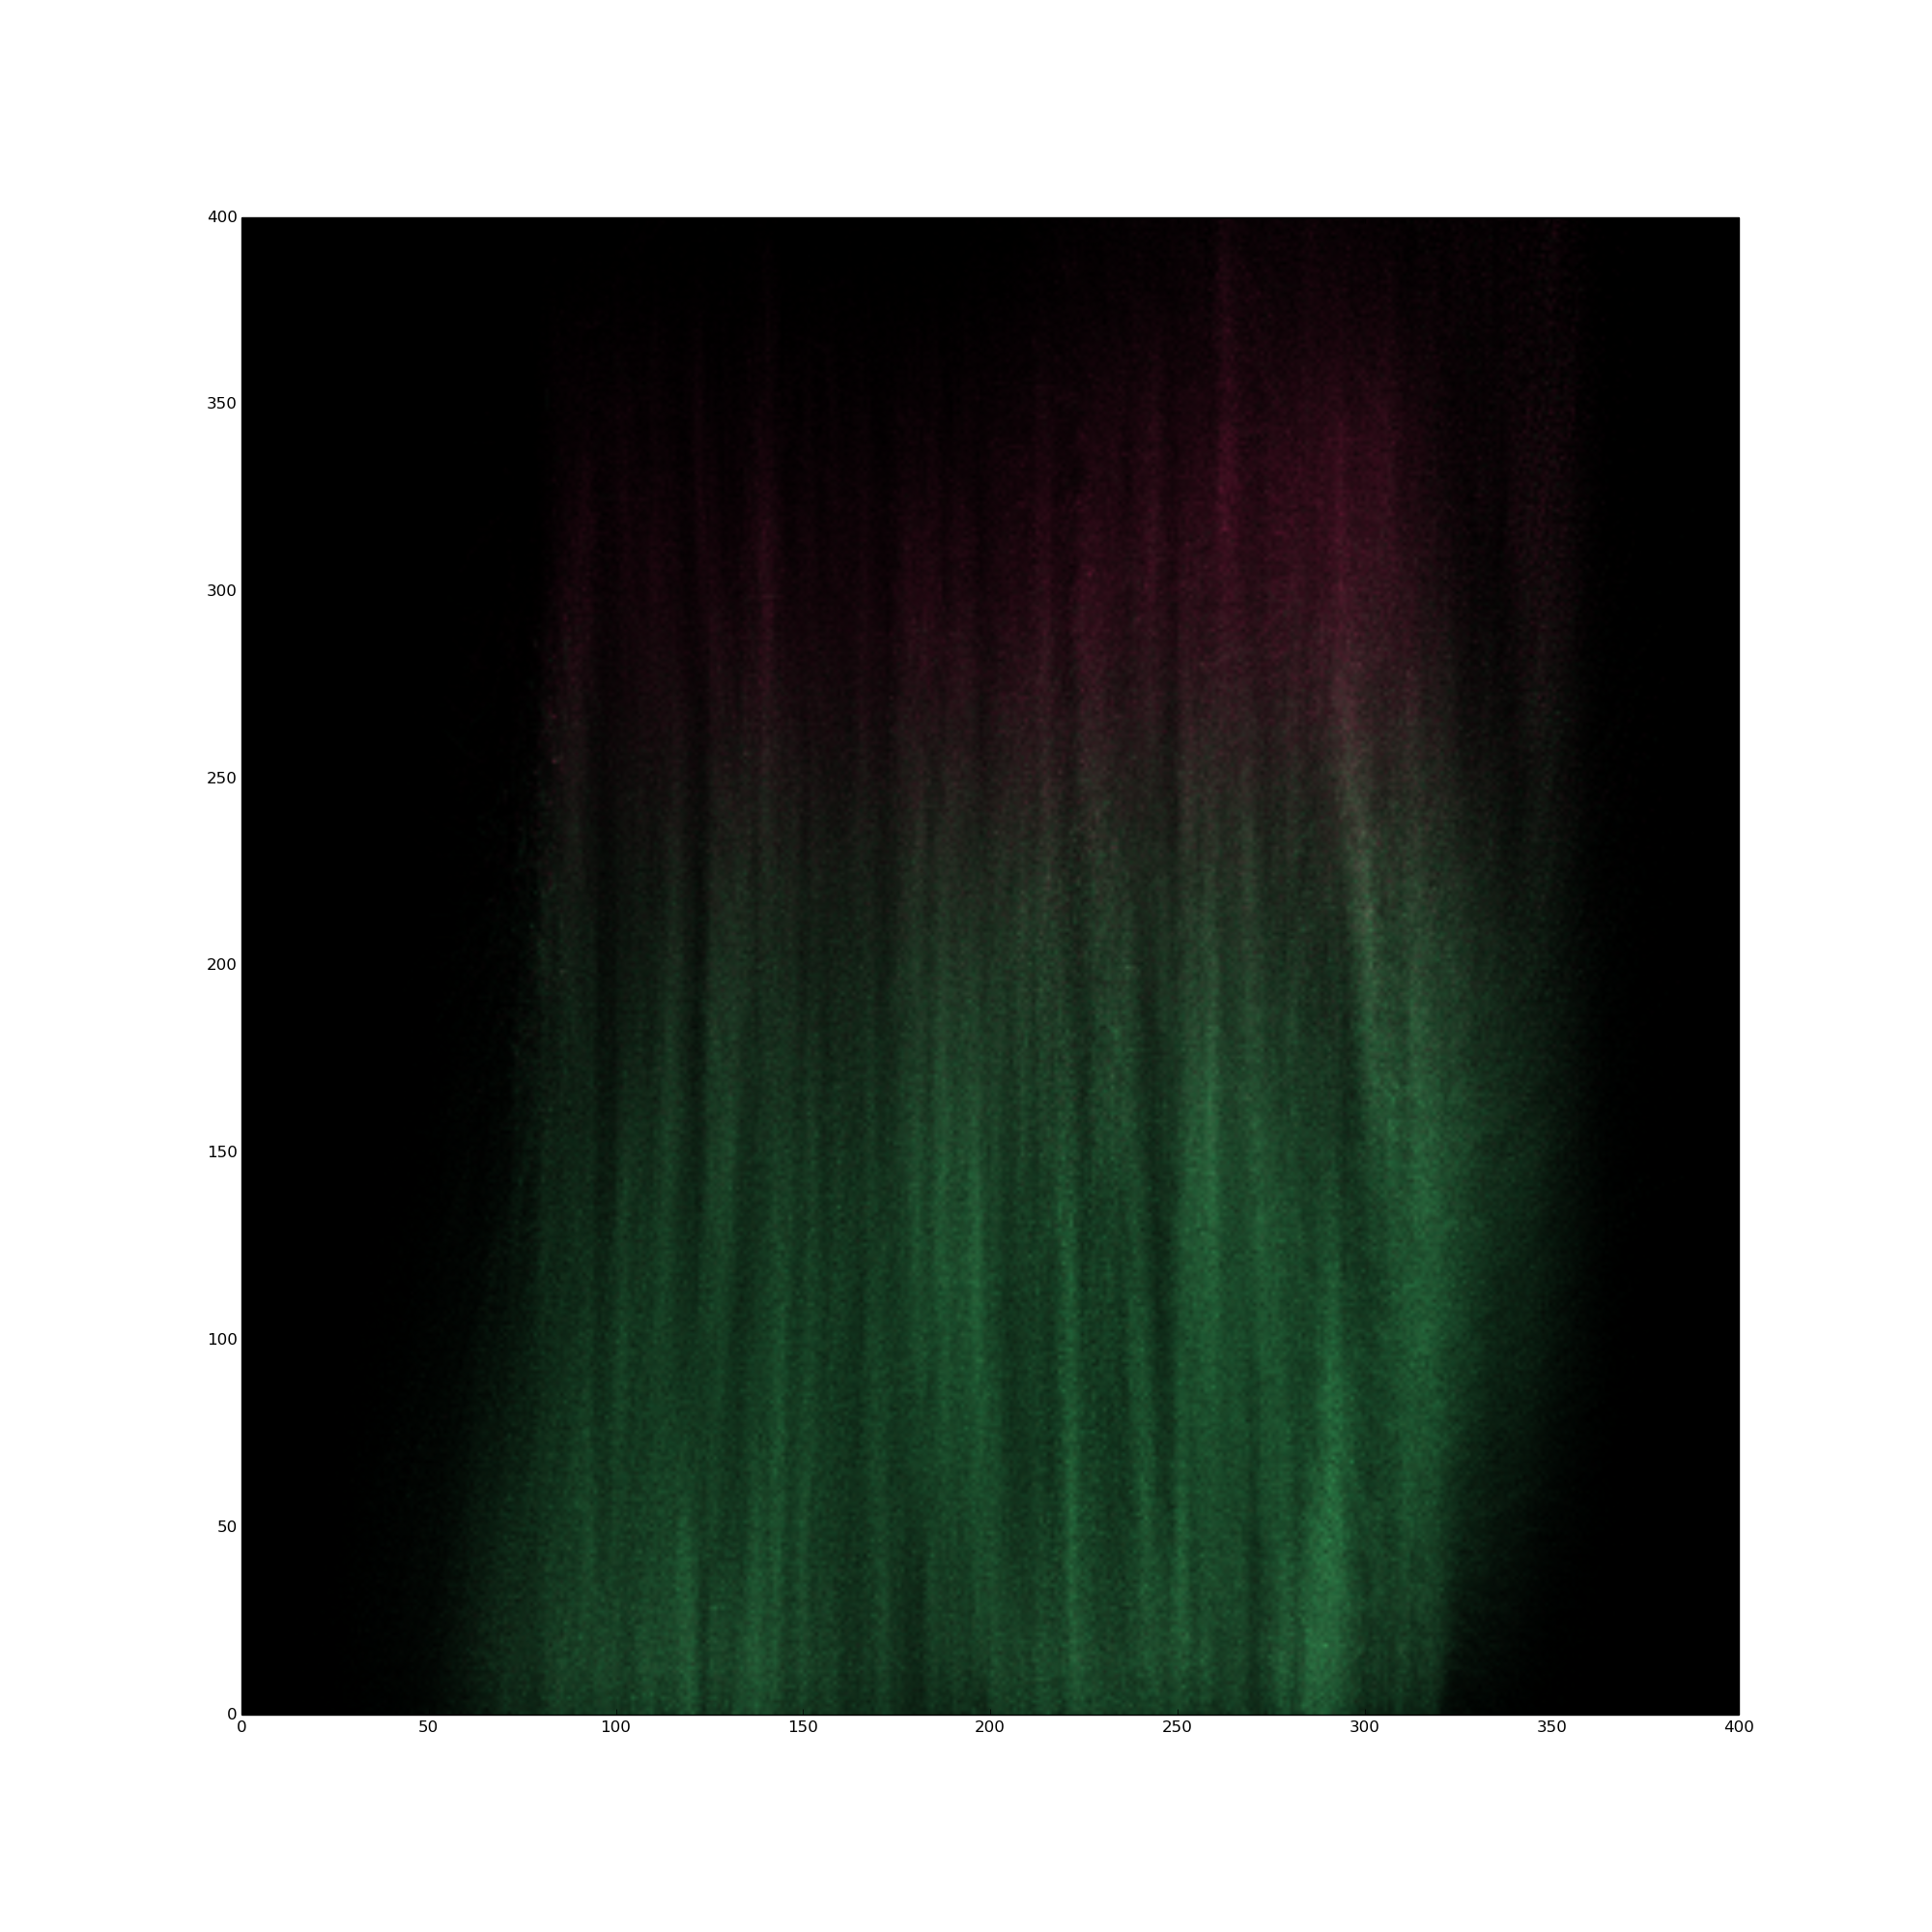
\includegraphics[width=0.75\textwidth]{img/Earth_thumbnail.png}
	}
\end{center}
\end{frame}





\section{Extension}
\begin{frame}{Extension}
\begin{itemize}
\item Baranoski's goal was to produce photorealistic \emph{images}, not necessarily give a realistic physical representation of the Aurora.
\item I want to see how close my model matches the real Aurora, in terms of energy
\end{itemize}
\end{frame}






\begin{frame}
  \begin{itemize}
  \item Every photon emission causes energy to be deposited into the system ($\Delta E = hc/\lambda$). We can compare with atmospheric measurements:
  \end{itemize}
\begin{center}
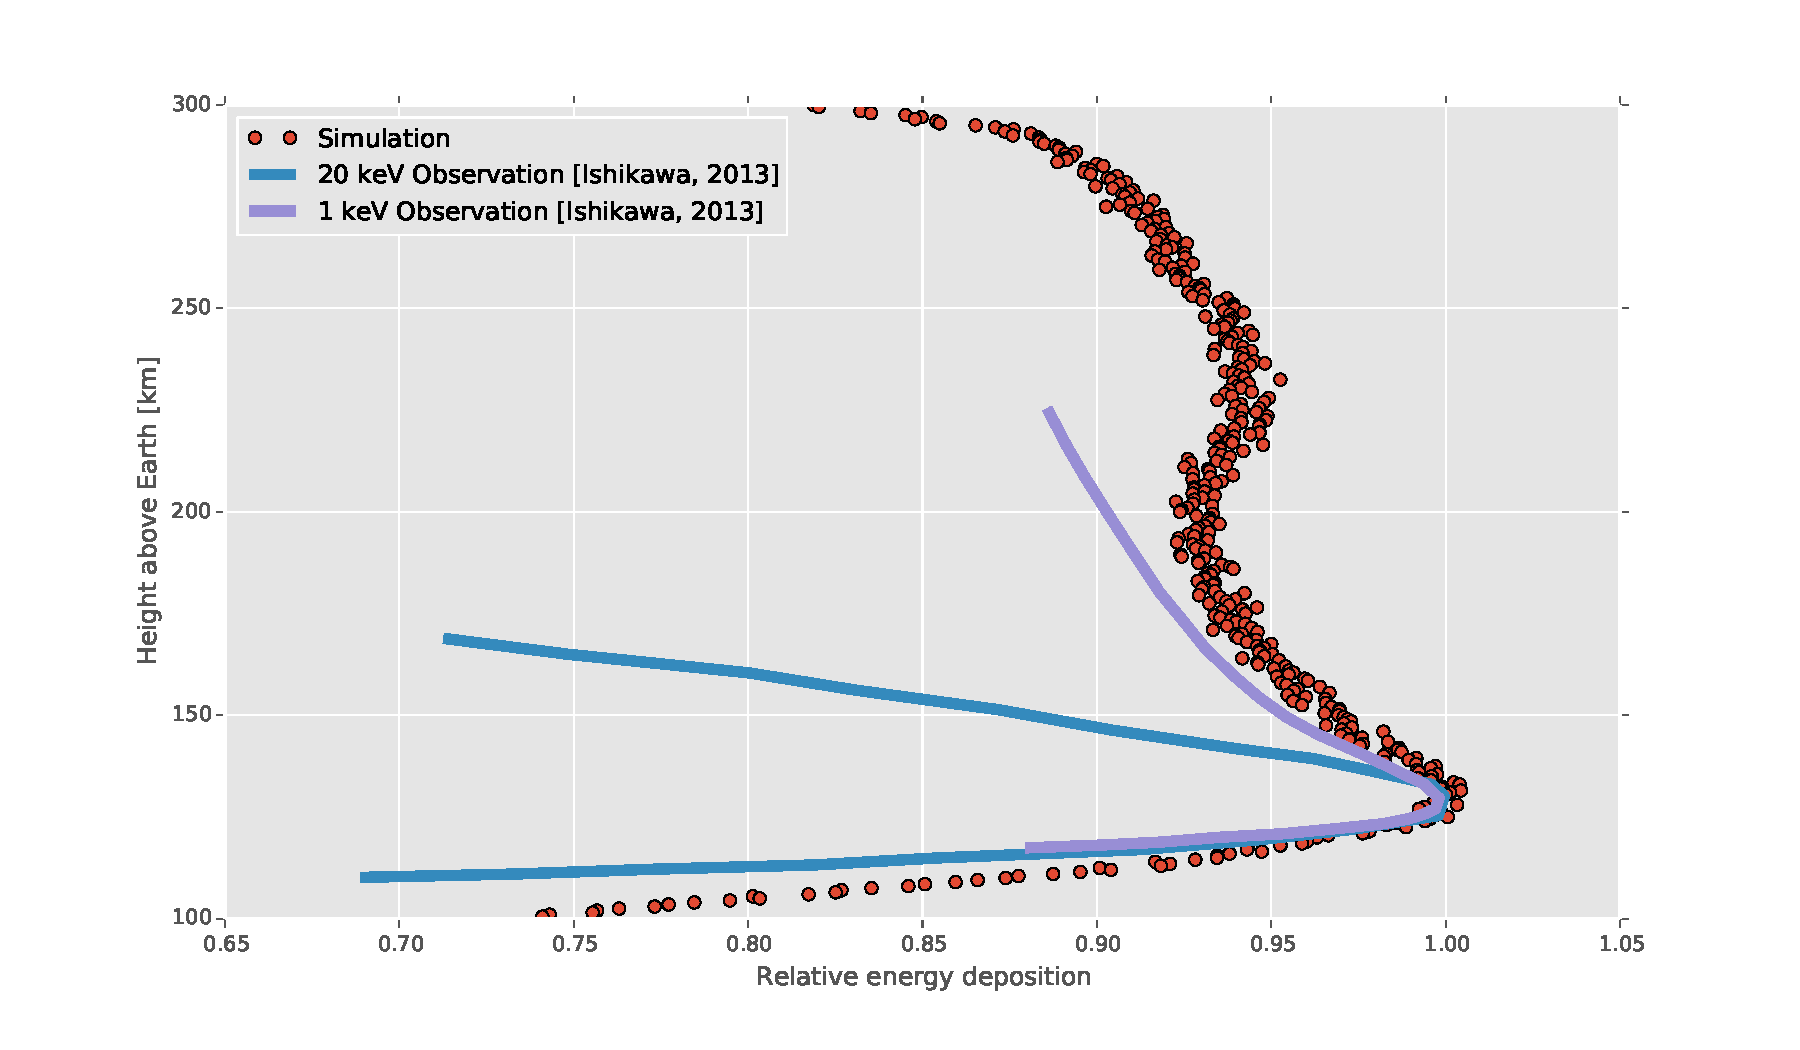
\includegraphics[width=\textwidth]{img/energy_deposition.pdf}
\end{center}
\end{frame}




\begin{frame}
  \begin{itemize}
  \item This could be improved by adding in more features that I neglected such as scattering, ionosphere fluid dynamics.
  \end{itemize}
\begin{center}
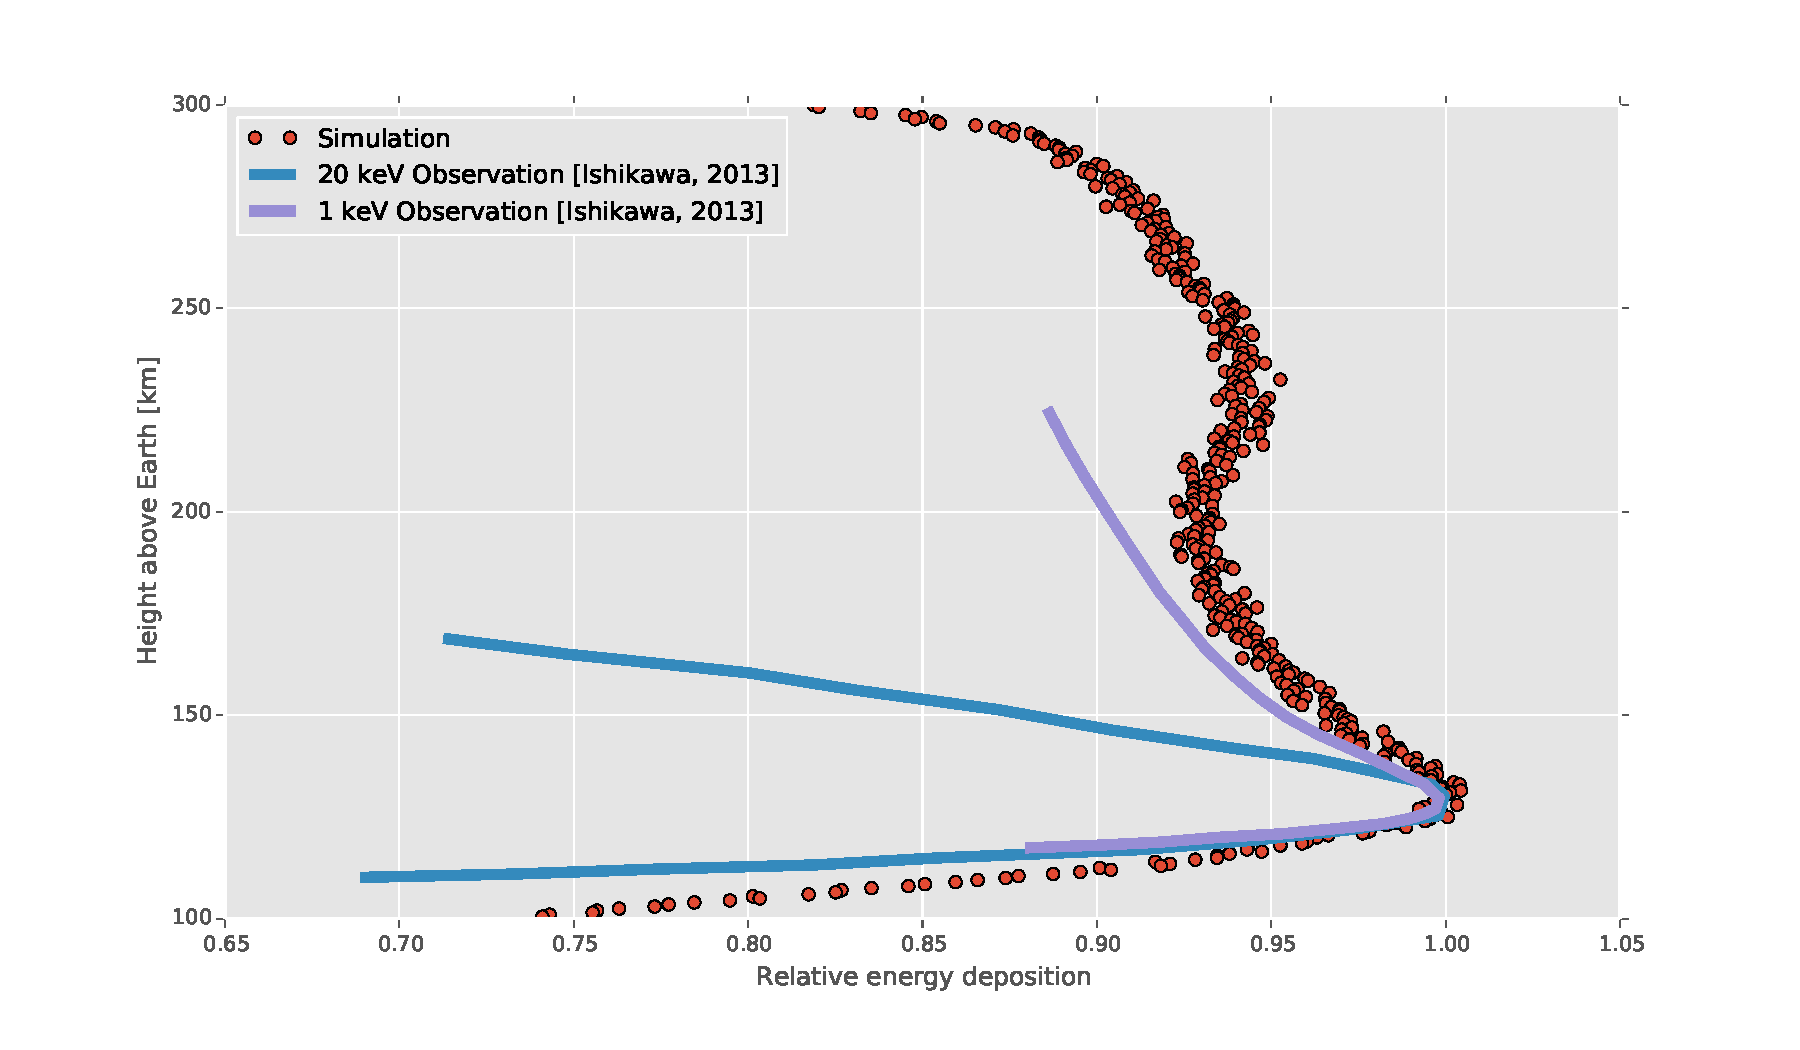
\includegraphics[width=\textwidth]{img/energy_deposition.pdf}
\end{center}
\end{frame}



\begin{frame}{Charge density}
\begin{center}
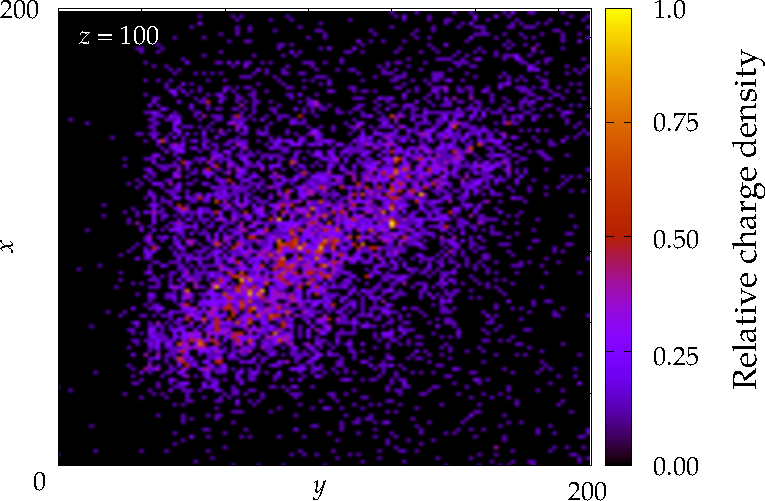
\includegraphics[width=0.8\textwidth]{img/charge_density.pdf}
\end{center}
\end{frame}







\begin{frame}{Aurora on Io}
  \begin{itemize}
    \item Jupiter's moon Io has intense Aurora, thousands of times more energetic than Earth's
    \item Atmosphere composed of SO$_2$ from volcanic activity
    \item 3 main emission wavelengths: 450 nm, 335 nm \& 300 nm
  \end{itemize}  \vfill
	\begin{center}
		
\includegraphics[width=0.685\textwidth]{img/io_spect.pdf}
	\end{center}
\end{frame}



\begin{frame}
\begin{columns}[onlytextwidth]
  \begin{column}{0.5\textwidth}
  \begin{itemize}
  
 \item Magnetic field of Io dominated by magnetic field of Jupiter
\subitem{Larger magnetic field in $z$ direction }
\item Spreads electrons more, hides the banding structure
  \end{itemize}
  \end{column}
  \begin{column}{0.05\textwidth}
  \end{column}
  \begin{column}{0.5\textwidth}
    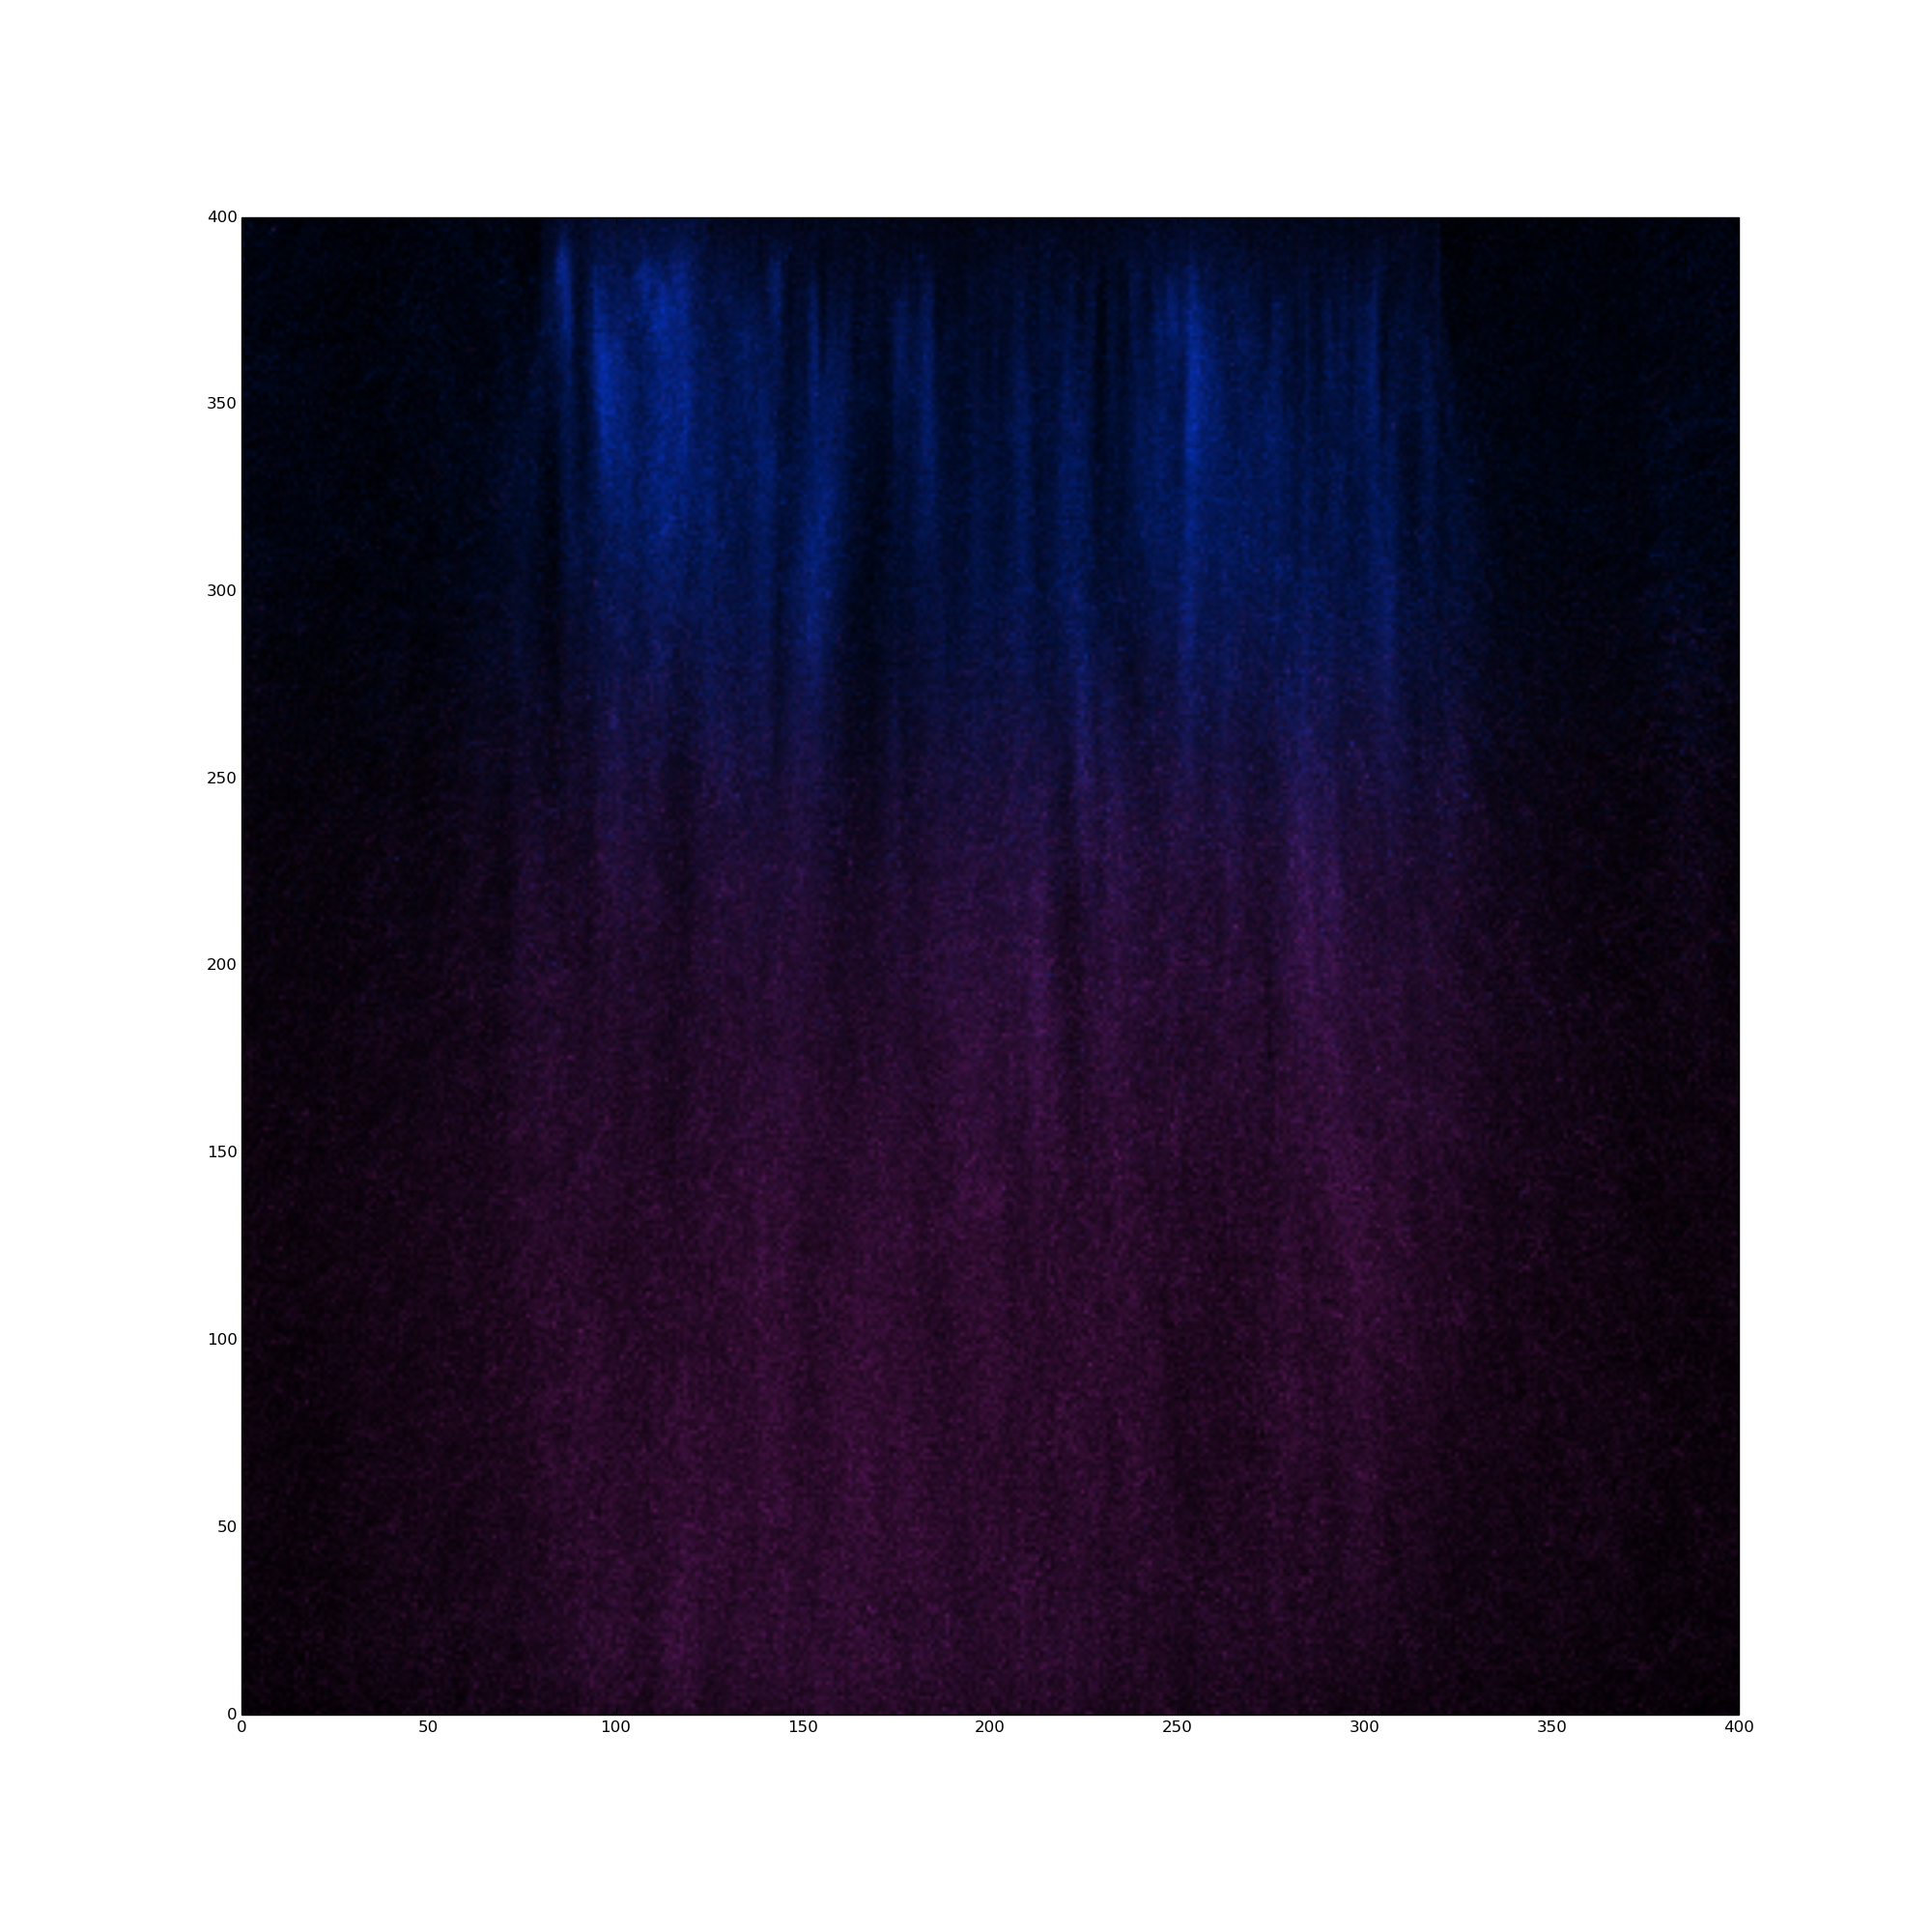
\includegraphics[width=\textwidth]{img/io_first.png}\\
  \end{column}
\end{columns} 
\end{frame}




\begin{frame}
\begin{center}
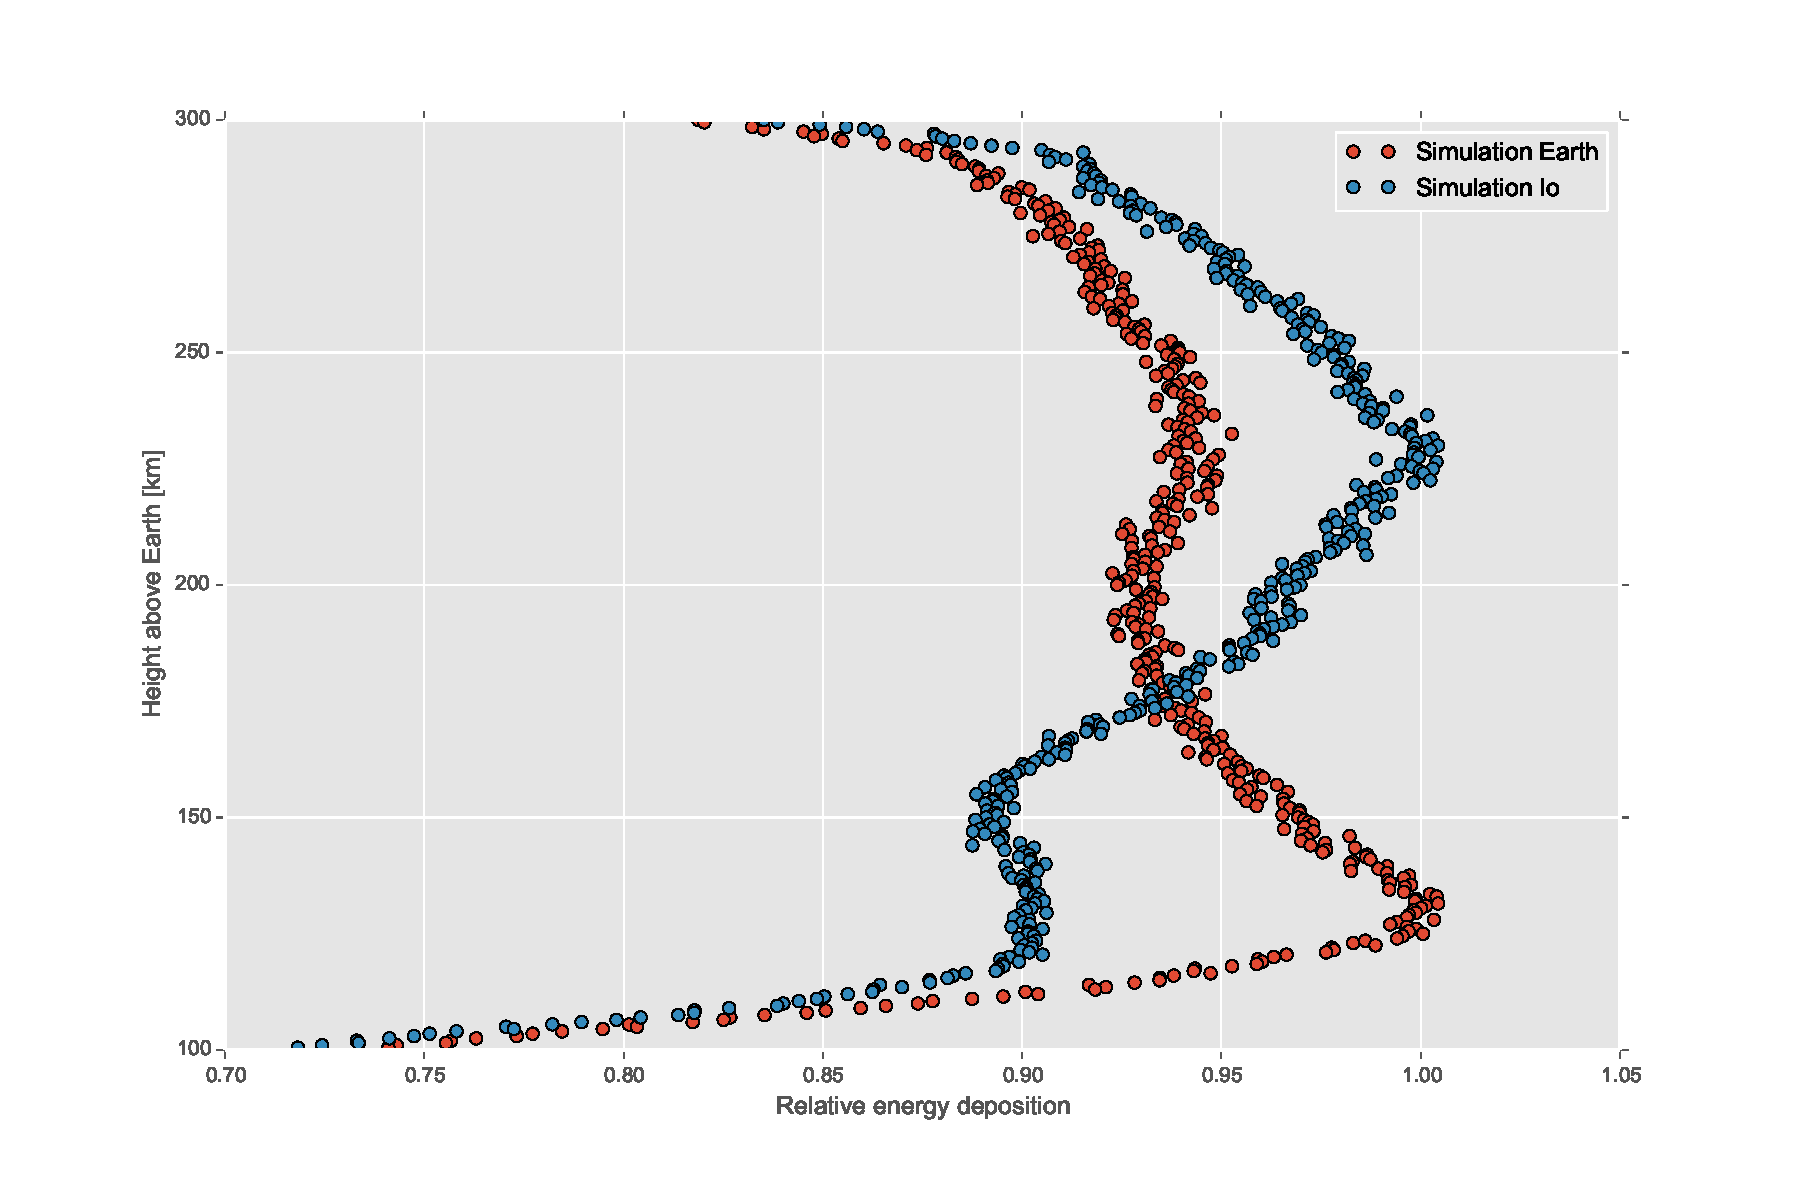
\includegraphics[width=1.0\textwidth]{img/energy_deposition_Earth_vs_io.pdf}
\end{center}
\end{frame}



\begin{frame}
\begin{center}
\href{run:/home/kmills/Dropbox/3.AdvancedTopics/AdvancedTopics/project/AuroraSim/presentation/vid/Io_1.mkv}{
	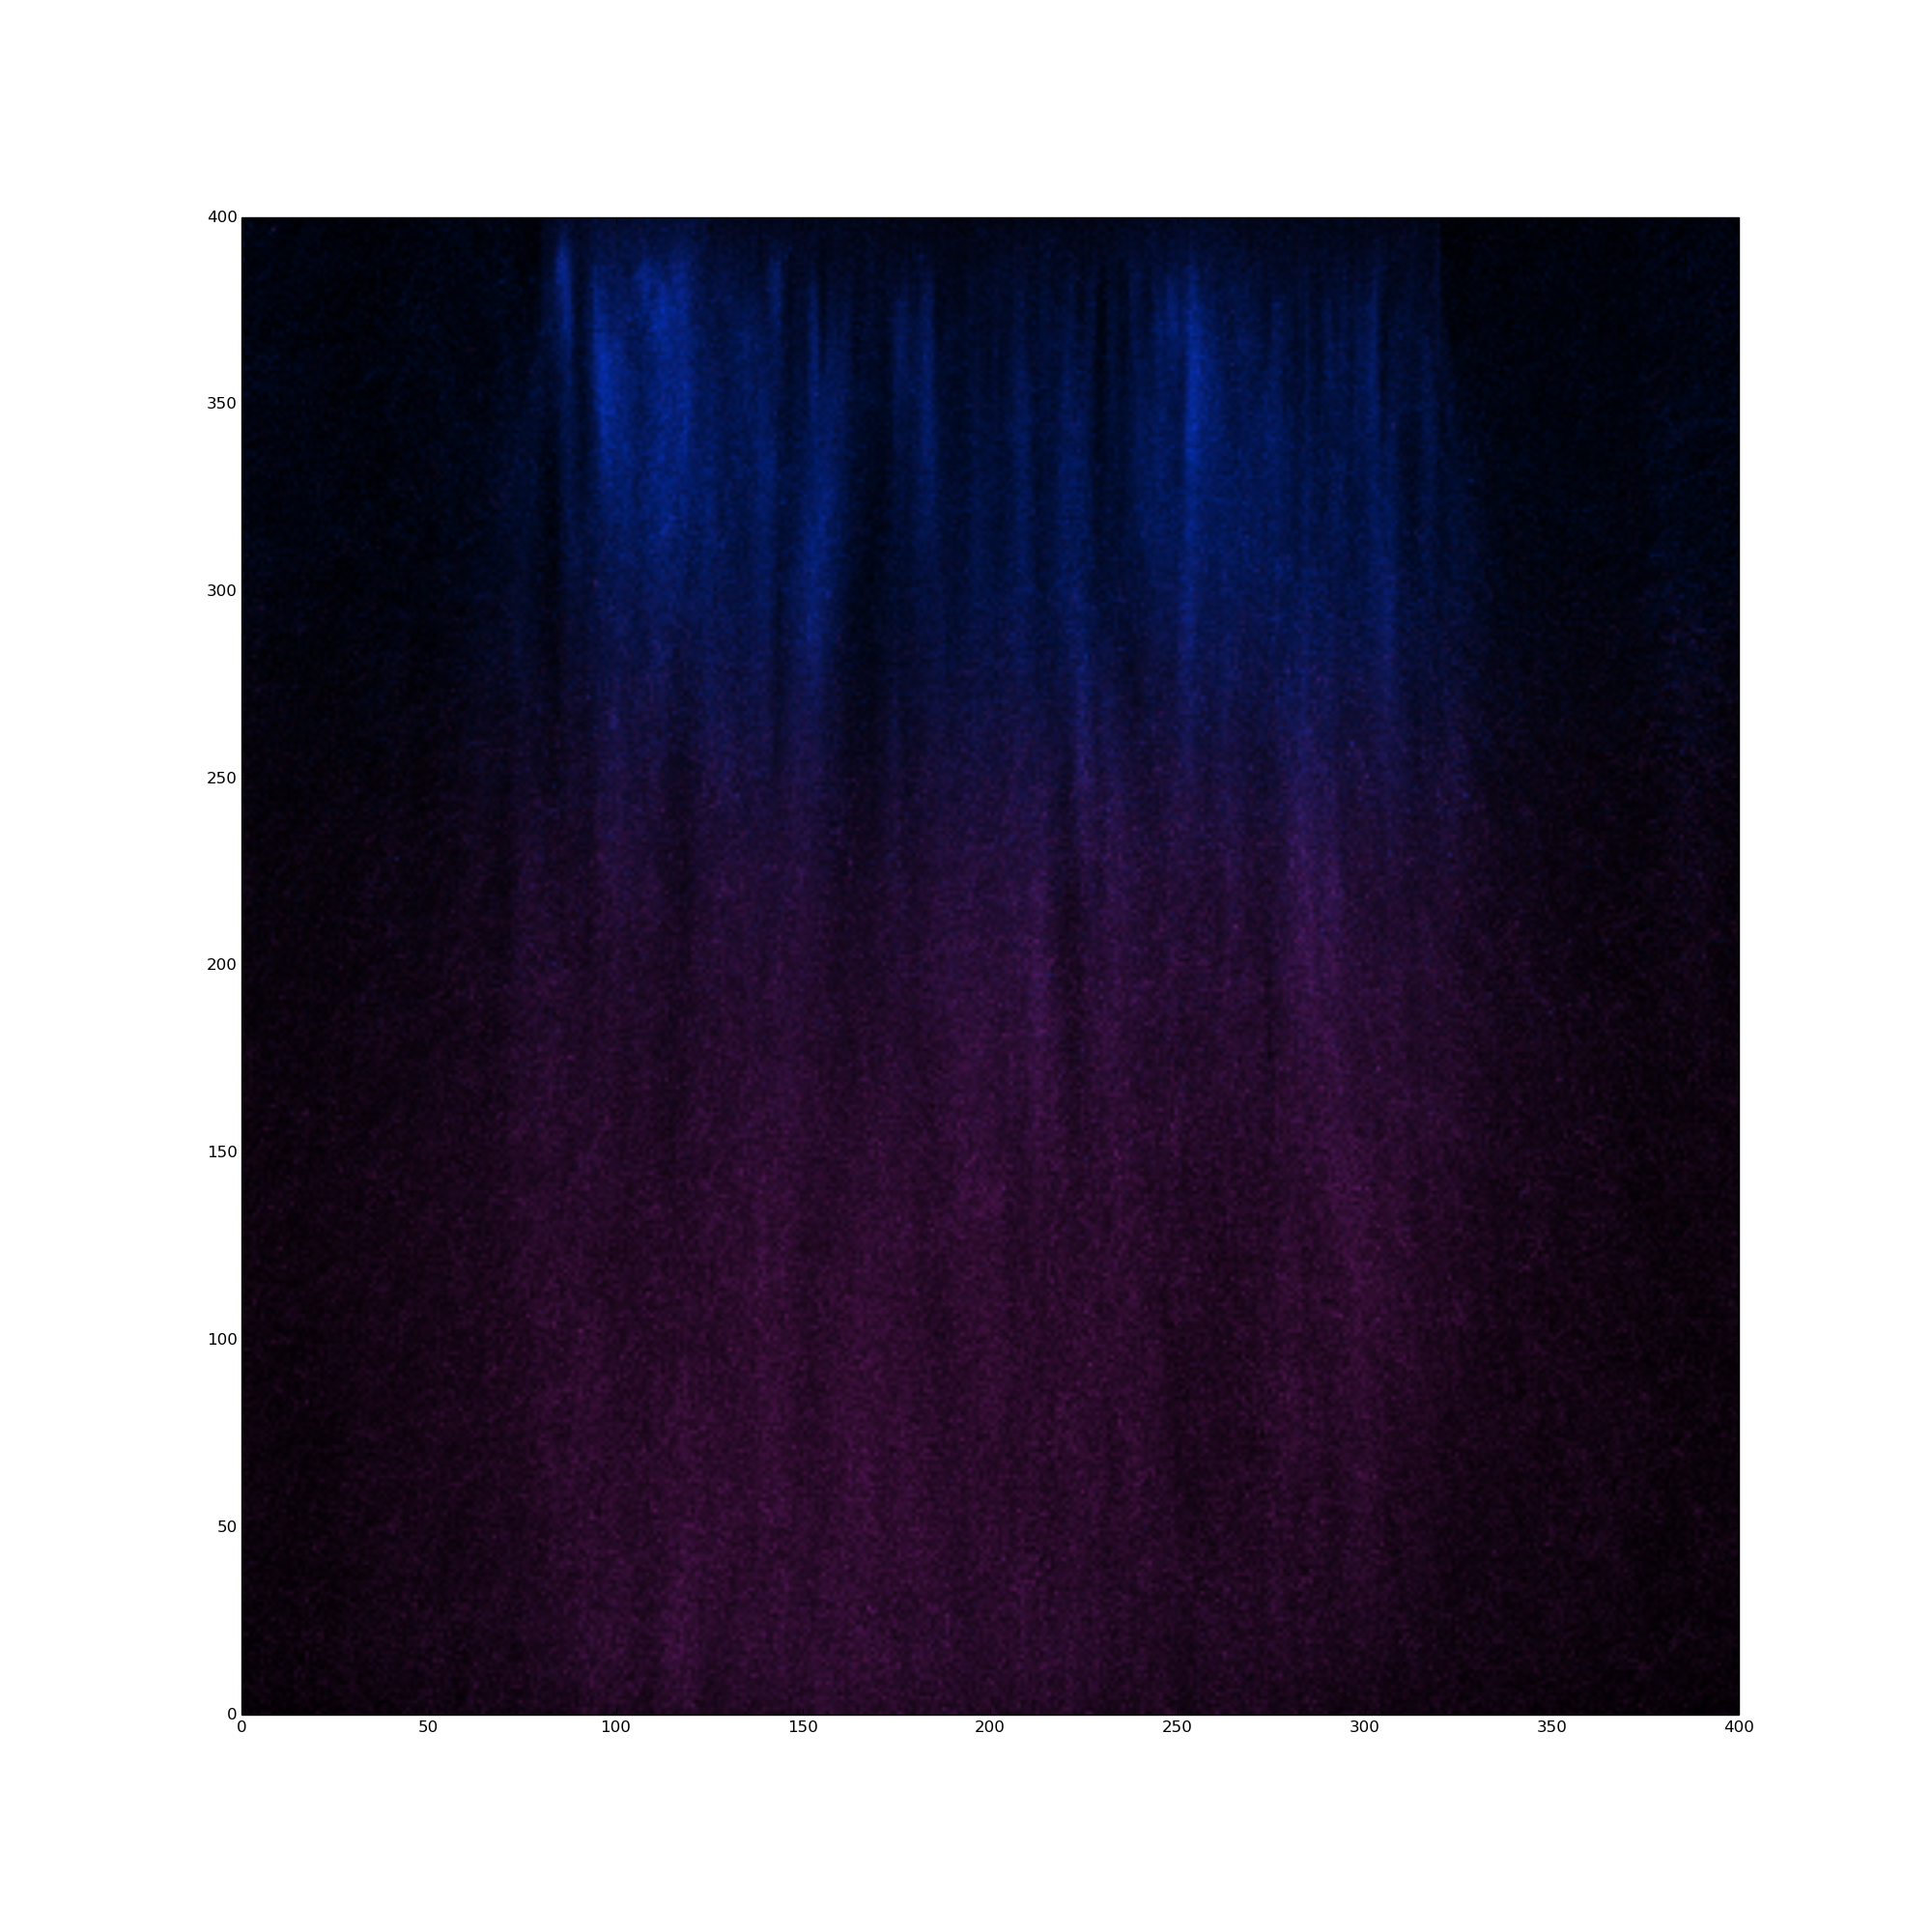
\includegraphics[width=0.75\textwidth]{img/io_first.png}
	}
\end{center}
\end{frame}



\begin{frame}

\end{frame}



\end{document}
